%
% Niniejszy plik stanowi przykład formatowania pracy magisterskiej na
% Wydziale MIM UW.  Szkielet użytych poleceń można wykorzystywać do
% woli, np. formatujac wlasna prace.
%
% Zawartosc merytoryczna stanowi oryginalnosiagniecie
% naukowosciowe Marcina Wolinskiego.  Wszelkie prawa zastrzeżone.
%
% Copyright (c) 2001 by Marcin Woliński <M.Wolinski@gust.org.pl>
% Poprawki spowodowane zmianami przepisów - Marcin Szczuka, 1.10.2004
% Poprawki spowodowane zmianami przepisow i ujednolicenie 
% - Seweryn Karłowicz, 05.05.2006
% Dodanie wielu autorów i tłumaczenia na angielski - Kuba Pochrybniak, 29.11.2016

% dodaj opcję [licencjacka] dla pracy licencjackiej
% dodaj opcję [en] dla wersji angielskiej (mogą być obie: [licencjacka,en])
\documentclass[licencjacka]{pracamgr}

\usepackage{graphicx,xcolor}

% Dane magistranta:
%\autor{Imię Nazwisko}{123456}


% Dane magistrantów:
\autor{Daniel Gutowski}{372207}
\autori{Jakub Kuklis}{371125}
\autorii{Adrian Naruszko}{371233}
\autoriii{Filip Plata}{371335}

\title{Modernizacja architektury autorskiego CMS firmy E-point}


%\tytulang{An implementation of a difference blabalizer based on the theory of $\sigma$ -- $\rho$ phetors}

%kierunek: 
% - matematyka, informacyka, ...
% - Mathematics, Computer Science, ...
\kierunek{informatyka}

% informatyka - nie okreslamy zakresu (opcja zakomentowana)
% matematyka - zakres moze pozostac nieokreslony,
% a jesli ma byc okreslony dla pracy mgr,
% to przyjmuje jedna z wartosci:
% {metod matematycznych w finansach}
% {metod matematycznych w ubezpieczeniach}
% {matematyki stosowanej}
% {nauczania matematyki}
% Dla pracy licencjackiej mamy natomiast
% mozliwosc wpisania takiej wartosci zakresu:
% {Jednoczesnych Studiow Ekonomiczno--Matematycznych}

% \zakres{Tu wpisac, jesli trzeba, jedna z opcji podanych wyzej}

% Praca wykonana pod kierunkiem:
% (podać tytuł/stopień imię i nazwisko opiekuna
% Instytut
% ew. Wydział ew. Uczelnia (jeżeli nie MIM UW))
\opiekun{mgr. Krzysztofa Wojciecha Ciebiery\\
  Instytut Informatyki\\
  }

% miesiąc i~rok:
\date{Kwiecień 2018}

%Podać dziedzinę wg klasyfikacji Socrates-Erasmus:
\dziedzina{ 
%11.0 Matematyka, Informatyka:\\ 
%11.1 Matematyka\\ 
%11.2 Statystyka\\ 
11.3 Informatyka\\ 
%11.4 Sztuczna inteligencja\\ 
%11.5 Nauki aktuarialne\\
%11.9 Inne nauki matematyczne i informatyczne
}

%Klasyfikacja tematyczna wedlug AMS (matematyka) lub ACM (informatyka)
\klasyfikacja{D. Software\\
  D.127. Blabalgorithms\\
  D.127.6. Numerical blabalysis \\
  ??TODO
  }

% Słowa kluczowe:
\keywords{CMS, Java, ORM, rendering, modernizacja, Jooq, Gatling, Caffeine, cache}

% Tu jest dobre miejsce na Twoje własne makra i~środowiska:
\newtheorem{defi}{Definicja}[section]

% koniec definicji

\begin{document}

\maketitle

%tu idzie streszczenie na strone poczatkowa
\begin{abstract}
  W~pracy przedstawiamy opis współpracy w firmą e-point.
  Produktem nad którym pracowaliśmy, jest autorski
  system CMS. W momencie rozpoczęcia współpracy miał on strukturę monolitu.
  Naszym zadaniem było napisanie mikroserwisów umożliwiających
  dalszą modernizację i modularyzację tego produktu. 
  Ostatecznie zajmowaliśmy się komponentami odpowiadającymi za dostęp do bazy danych oraz rendering.
\end{abstract}

\tableofcontents
%\listoffigures
%\listoftables

\chapter*{Wprowadzenie}
\addcontentsline{toc}{chapter}{Wprowadzenie}
    
Z biegiem lat technologia rozwija się coraz szybiej. Stwierdzenie to sprawdza się od wieków, ale jego implikacje stają się znacznie poważniejsze w miarę rozwoju cywilzacji. Powszechne wcześniej rozwiązania i reguły prędko stają się przestarzałe i wymagają renowacji, co często oznacza całkowitą zmianę podejścia czy redefinicję problemu.

\vspace{1mm}

Nie inaczej jest w przypadku usług sieciowych, szczególnie żywej dziedziny w czasach powszechnego Internetu i postępującej globalizacji. Świadczy o tym chociażby mnogość frameworków i technik wykorzystywanych przy ich tworzeniu, nieustannie ewoluujących w miarę odkrywania wad w używanych wcześniej wersjach. Przed problemem modernizacji swojego systemu stanęła m.in. firma E-point, które to zadanie powierzyła w części naszemu zespołowi.

\vspace{1mm}

W szczególności, zajmowaliśmy się implementacją dwóch mikroserwisów:
\begin{enumerate}
\item DataAPI - RESTowa aplikacja integrująca bazę danych aktualnego CMSa z nowym mechanizmem renderingu.
\item Element odpowiedzialny za rendering serwisów internetowych i związana z nim architektura.
\end{enumerate}

\chapter{Zarys sytuacji i problemu}

\begin{center}

\includegraphics[scale=0.62]{logo.JPG}
\end{center}

\section{Firma E-point}

E-point to polskie przedsiębiorstwo zajmujące się tworzeniem oprogramowania, dostarczające systemy internetowe dla międzynarodowych korporacji oraz usługi w modelu SaaS (software as a service). Założone w 1996 roku, działa nieprzerwanie od ponad 20 lat, otrzymując za swoją działalność liczne nagrody i wyróżnienia od przedstawicieli branży technologicznej. Jej klientami są największe firmy polskie i zagraniczne, takie jak ING Bank Śląski, Bank BGŻ BNP Paribas czy Amway.

Firma koncentruje się na następujących sektorach:
\begin{itemize}
\item systemy e-business – aplikacje mające na celu sprzedaż produktów i usług oraz zapewnienie obsługi klientów i partnerów przez internet; sklepy internetowe, bankowość elektroniczna, eCRM, systemy obsługi zamówień;
\item  portale korporacyjne – systemy mające na celu udostępnianie informacji na zewnątrz i wewnątrz organizacji – serwisy WWW, portale wewnętrzne, extranety;
\item aplikacje mobilne aplikacje i serwisy na smartfony i tablety;
\item systemy e-wniosków – rozwiązania zorganizowane wokół zagadnienia zbierania i przetwarzania wniosków (formularzy elektronicznych);
\item systemy mające na celu obsługę wybranych procesów biznesowych w organizacji – rejestry, wsparcie sprzedaży, operacyjne CRM, e-learning.
\end{itemize}

W czasie tylu lat istnienia E-point wypuścił na rynek wiele swoich własnych produktów, m.in. kreator stron mobilnych ActiveMobi, modeler baz danych Vertabelo czy OneWebSQL, pierwsze polskie narzędzie do mapowania obiektowo-relacyjnego – sposobu odwzrowoania obiektowej architektury systemu informatycznego na bazę danych o relacyjnym charakterze. Nasze zadanie związane były z wewnętrznym CMS, używanym do zarządzania danymi i renderowania odpowiednich treści w serwisach internetowych klientów firmy.

\section{ACN}

ACN - wewnętrzny CMS (Content Management System) - to jeden z największych produktów firmy. Odpowiada za cały proces utrzymywania, przygotowania i serwowania danych serwisom internetowym. W momencie otrzymania zapytania load balancer decyduje o przekierowaniu go do odpowiednio odciążonego serwera. Request trafia do ACN, który sprawdza uprawnienia dostępu, a po ich pomyślnej weryfikacji wyciąga dostępne komponenty z cache’u, a o informacje potrzebne pozostałym odpytuje bazę danych. W dalszej kolejności renderowane są niecache’owalne elementy strony oraz te nieobecne w danym momencie w cache’u. Po wygenerowaniu wszystkich potrzebnych komponentów strona jest serwowana użytkownikowi.

\vspace{1mm}

[ schemat ACN ]

\section{Problemy obecnej architektury}
Dotychczas ACN stanowił monolit. Jest to produkt tworzony od wielu lat, stale rozwijany i rosnący. W samej bazie danych część zmian podyktowana była indywidualnymi wymaganiami klientów, przez co stała się ona mało przejrzysta i trudna w utrzymaniu. Duża wielkość systemu sprawia, że jego modyfikacja jest uciążliwa – zachowanie spójności wszystkich usług przy nawet pozornie małych zmianach wymaga wielu godzin pracy nad kodem. Utrudniona jest także lokalizacja błędów w systemie, brak modułowości oznacza konieczność przeszukiwania znacznie większej ilości kodu w celu wykrycia usterki.

\vspace{1mm}

W związku z powyższym, firma postanowiła dostosować swój produkt do bardziej nowoczesnego podejścia do problemu. Tak pojawił się pomysł przynajmniej częściowego wydzielenia funkcjonalności ACN do osobnych mikroserwisów. Implementacja dwóch z nich, elementu łączącego aplikację z bazą danych oraz serwisu renderującego komponenty strony, została przydzielona naszemu zespołowi.

\chapter{Koncepcja}
	
\section{Początek prac – inny projekt}

Założenia naszego projektu nie były od początku jasne. Pierwotnie mieliśmy zająć się w zasadzie innym zadaniem – zaimplementowaniem personalizacji treści serwisów internetowych na podstawie aktywności ich użytkowników. Miało to pozwolić przede wszystkim na bardziej trafne wyświetlanie ofert i reklam. Po wstępnej konfiguracji dostępów i tunelowania zdążyliśmy stworzyć podstawową architekturę aplikacji i skonfigurować narzędzie deweloperskie na AWS, kiedy okazało się, że rozwój produktu zostaje wstrzymany ze względu na problemy z jego sprzedażą. Wtedy też wyklarowało się, że nasz projekt będzie w całości poświęcony modernizacji aktualnie funkcjonującego systemu.

\section{Ostateczny projekt}
	
Rozwiązanie zaproponowane i wdrażane przez firmę ma opierać się na stylu programowania REST, tj. wykorzystującym predefiniowane bezstanowe operacje, co pozwala osiągać dużą wydajność, modułowość i niezawodność aplikacji. Docelowo pojawić mają się następujące mikroserwisy:
\begin{itemize}
\item frontend - przyjmowanie zapytań i serwowanie stron WWW;
\item rendering - tworzenie stron na podstawie szablonów, wykorzystuje usługi udostępniane przy pomocy serwisu Registry;
\item AC Data API - abstrakcja bazy danych, udostępnia tylko niezbędne renderingowi dane;
\item registry - rejestr wewnętrznych i zewnętrznych usług takich jak podmiana tagów, personalizacja treści;
\item ACN - dotychczasowa aplikacja implementująca niektóre usługi, w końcowym etapie ma zniknąć;
\end{itemize}

\begin{figure}\label{architektura}
	\centering
	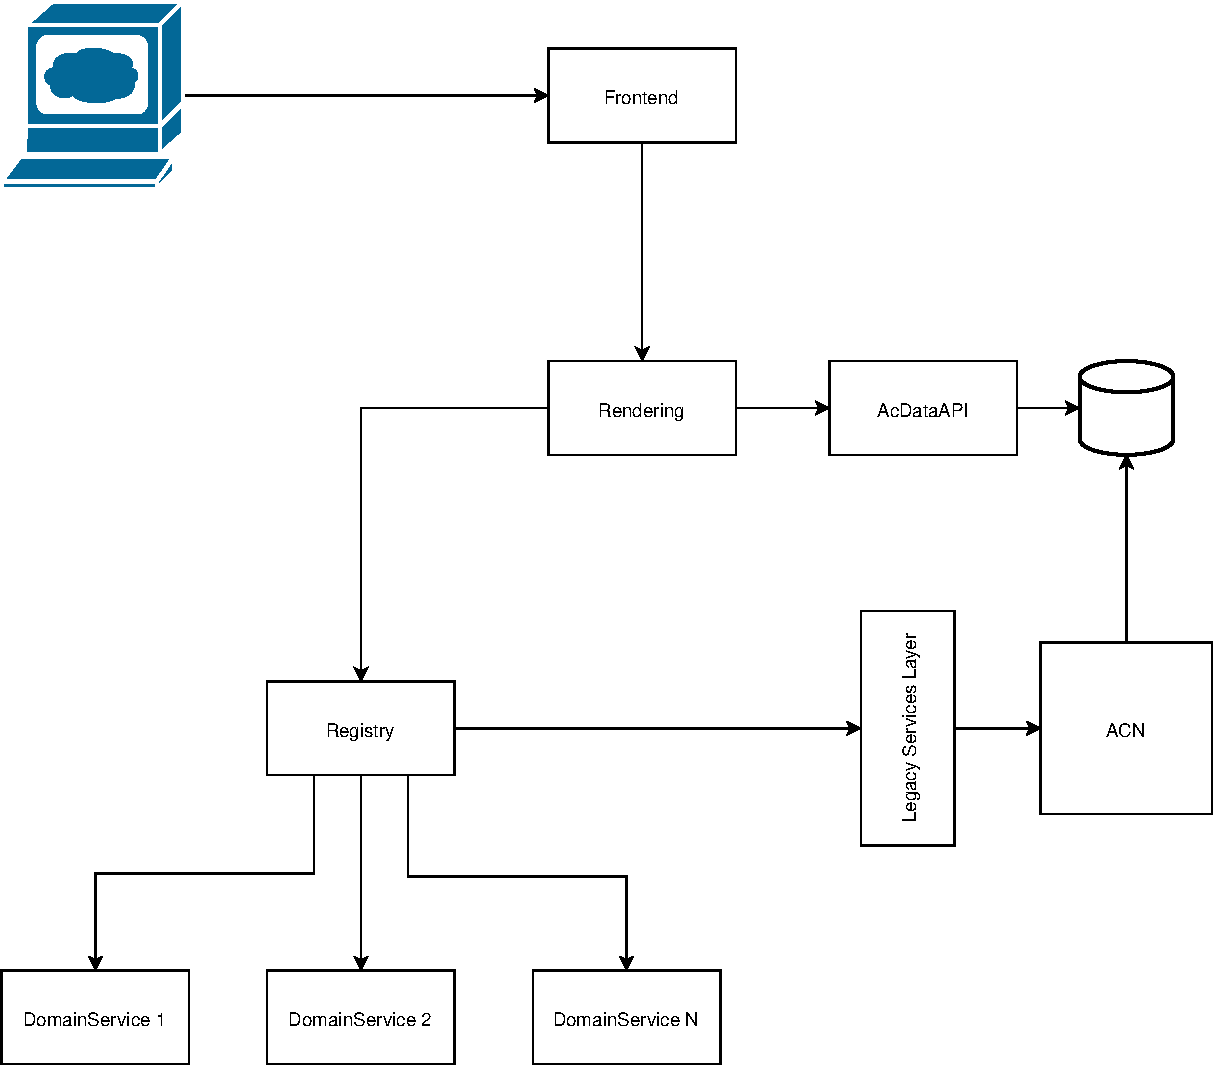
\includegraphics[scale=0.82]{architecture.pdf}
	\caption{Schemat wydzielonych aplikacji}
\end{figure}

Nasza grupa zajmowała się elementami Data API oraz serwisem renderującym. W przypadku tego drugiego, część pracy stanowiło wprowadzenie zmian w samym ACN, związanych z dostosowywaniem narzędzia do nowej koncepcji schematu renderowania.


\chapter{AC Data API}

\section{Mikroserwis}

Obsługa serwisów internetowych wymaga niezawodnego i bezpiecznego sposobu łączenia z bazą danych, stąd pojawia się potrzeba wydzielenia odpowiednigo mikroserwisu odpowiedzialnego za to zadanie. E-point korzysta z tradycyjnych relacyjnych baz danych, co pociąga za sobą stosowanie ORM przy wyciąganiu danych do dalszego przetwarzania.

\vspace{1mm}

Aplikacja Data API ma udostępniać dane z bazy danych ACN dla komponentów w nowej architekturze. Będzie to jeden z najczęściej odpytywanych serwisów, w związku z czym jego wydajność oraz dostępność jest krytyczna dla sprawnego i poprawnego działania całej usługi.

\section{Założenia}

Aplikacja docelowo ma specyfikować oraz implementować kontrakt obslugi REST’owych endpointów, których nazwy składają się z wersji API oraz tytułu zapytania (np. /v1/language-version). Odpowiedzią na dane żądanie jest JSON zawierający odpowiednie dane z bazy.

\vspace{1mm}

Dane z bazy danych mają być zapisywane w odpowiednio inwalidowanym cache’u. Powodem inwalidacji może być upływ wyznaczonego czasu od zapisu czy powiadomienie o zmianie z innego serwisu połączonego z bazą danych (na ten moment funkcję tę pełni ACN).

\vspace{1mm}
	
API ma być dokładnie pokryte testami, zarówno poprawnościowymi, jak i wydajnościowymi. W pierwszej wersji nie jest wymagana żadna forma uwierzytelniania.

\section{Struktura bazy}

Baza danych składa się z wielu schematów. Głównym schematem jest schemat ‘master’. Przechowuje on informacje o klientach – organizacjach – korzystających z systemu firmy E-point. Dla każdego klienta tworzony jest schemat indentyfikowany jego kodem, zawierający np. informacje o użytkownikach zarejestrowanych w serwisach tegoż klienta. Dla każdego portalu zarządzanego przez organizację tworzony jest osobny schemat, w którym przechowywane są wszystkie dane dotyczące instancji portalu.

\pagebreak

\section{Użyte technologie}

Aplikacja została napisana w Javie w wersji 8 przy użyciu platformy Spring. Ostatecznie przy jej tworzeniu korzystaliśmy m.in. z:
\begin{itemize}
\item systemu automatycznego budowania Gradle;
\item pakietu Jooq (Java Object Oriented Querying), lekkiej biblioteki stworzonej pod ORM;
\item biblioteki Caffeine, służącej do cache’owania;
\item produktu Logstash i powiązanych z nim narzędzi takich jak Elasticsearch czy Kibana, służących do monitorowania działania aplikacji;
\item platformy Docker z postgresem do testowego deploymentu aplikacji;
\item frameworku Gatling, stosowanego przy tworzeniu i wykonywaniu scenariuszy testów wydajnościowych;
\item funkcjonalności związanych z IntelliJ IDEA.
\end{itemize}

\chapter{Praca nad AC Data API}

\section{Iteracja nr 1}

W pierwszej iteracji do generowania klas Javy na podstawie schematów z bazy danych użyliśmy pakietu Jooq. Zaprezentowany przez nas przykład rozwiązania oparty bardzo bezpośrednio na Jooqu został odrzucony przez naszych przełożonych ze względu na ujawnione braki w architekturze rozwiązania. Problematyczne okazało się m.in. zapewnienie ścisłego, sztywnego kontraktu przez API przy zmianach schematów w bazie danych.

\vspace{1mm}

Ujawnione wady wcześniejszej koncepcji spowodowały przestój w pracach związany z dyskusją nad możliwościami rozwiązania wykrytych problemów. Po dogłębnej analizie dostępnych narzędzi i prezentowanych przez nas demonstracyjnych kawałków kodu nasz przełożony zdecydował się na pozostaniu przy pakiecie Jooq, z tą różnicą, że warstwa aplikacji zależna od Jooq miała zostać wydzielona od pozostałej części kodu, niezależnej od sposobu dostępu do bazy danych.

\vspace{1mm}

W tej wersji do monitorowania aktywnych instancji aplikacji użyliśmy gotowego, dedykowanego narzędzia spring-boot-admin. Niestety, konfiguracja narzędzia okazała się tyleż prosta, co ograniczona. Nie mogąc spełnić wymogów firmy przy jego pomocy, zdecydowaliśmy się na inny produkt do monitorowania aplikacji.
	
\section{Iteracja nr 2}

Ta iteracja poświęcona była przede wszystkim na poprawne zaimplementowanie ORM oraz stworzenie potrzebnych endpointów. Przyjęliśmy architekturę podzieloną na kilka warstw odpowiedzialnych za wydzielone zadania. 

\vspace{1mm}

Najniższa z nich zapewnia bezpośredni dostęp do bazy danych poprzez Jooq. Druga warstwa zajmuje się dzieleniem danych klientów na schematy w bazie, zarządzaniem aktualnymi schematami. Następny poziom ukrywa działanie Jooq’a poprzez utworzenie obiektów domenowych. Ostatecznie wersjonowanie API poprzez javowe pakietowanie umożliwia zapewnienie kontraktu kompatybilnego wstecz nawet pomimo zmian schematu bazy daych.

\vspace{1mm}

Odpowiednie endpointy realizują zapytania potrzebne wyższym poziomom obsługi żądań do stron. Listę koniecznych na ten moment zapytań przygotowali nasi przełożeni. Wśród zaimplentowanych endpointów znajdują się m.in. zapytania pobierające wersje językowe, informacje o kliencie o zadanym identyfikatorze czy własności strony o zadanym id. Wszystkie te metody są obłożone testami poprawnościowymi w JUnit.

\section{Iteracja nr 3}

Mając zaimplementowaną strukturę aplikacji, przystąpiliśmy do zadań związanych z jej wydajnością. Pierwszym krokiem była konfiguracja cache’u. Na podstawie analizy dostępnych w internecie źródeł i benchmarków zdecydowaliśmy się na Caffeine, bardzo wydajną bibliotekę do cache’owania oparta na Javie 8.

\vspace{1mm}

Spring dobrze współdziała z różnymi frameworkami i Caffeine nie jest tu wyjątkiem. Wybór elementów do cache’owania odbywa się poprzez dodanie odpowiednich adnotacji przy cache’owanych funkcjach – model zmian w kodzie przy pomocy adnotacji to zresztą powszechny w Springu mechanizm.

\vspace{1mm}

Gotowy cache poddaliśmy testom wydajnościowym generowanym przy pomocy scenariuszy korzystających z Gatlinga.

\vspace{1mm}

Działanie całej aplikacji możemy monitorować, korzystając z Elastic Stacka. Wymaga on wprawdzie ręcznego wprowadzania reguł dla oczekiwanych statystyk i nie radzi sobie najlepiej z agregowanymi danymi, zapewnia za to pełną konfigurowalność. Narzędzia związane z Elastic Stackiem takie jak Kibana pozwalają nam na graficzną reprezentację zebranych statystyk, poniżej przykładowe wynikowe wykresy.

	[Wykresy z Kibany]

\chapter{Rendering}

\section{Spotkanie}

Po oddaniu ostatnich elementów Data API i przejściu przez etap recenzji odbyliśmy spotkanie w firmie dotyczące kontynuacji naszej współpracy. Przedstawiona została na nim wizja dalszego podziału ACN i wydzielenia z niego elementu renderującego.

\section{Dotychczasowy rendering}

W poprzedniej wersji renderowanie miało formę dwuetapową. W jednym z etapów renderowane były komponenty z ustawionym w bazie danych parametrem ‘noncacheable attributes’. Elementy te miały swoje wersje w cache’u zależne od parametru żądania (zazwyczaj) czy też ciasteczka pochodzącego z sesji. Całość renderowania wykonywania była przez ACN, co ograniczało wydajność systemu.

\vspace{1mm}

W rozwiązaniu wdrażanym przez firmę opisany wyżej postprocessing ma docelowo zniknąć. Naszym zadaniem było takie przystosowanie ACN, które pozwoliłoby na pozostawienie części renderingu przeglądarce użytkownika. Elementem tej pracy było zastąpienie wspomnianego wcześniej podejścia przez coś lepszego.

	[co lepszego? Na razie nie wiadomo]
	
\vspace{1mm}	
	
Dopiero po wykonaniu powyższego zadania mogliśmy przystąpić do pisania nowego komponentu renderującego.

\section{Iteracja nr 1}
	
Pierwszym etapem naszej pracy była konfiguracja środowiska potrzebnego do testowania wprowadzanych przez nas zmian. Ostatecznie postanowiliśmy trzymać całe środowisko na maszynie wirtualnej. Do obsługi serwera używany jest Apache oraz JBoss. Dla usprawnienia pracy korzystamy także z JRebela, narzędzia pozwalającego na aktualizowanie kodu i obserowanie zmian bez restartowania serwera.

\vspace{1mm}

W tym czasie nasi przełożeni przygotowywali zmiany w komponentach powiązanych z ACN, takich jak OneWeb, by umożliwić nam pracę nad serwisem renderującym. Jedną z istotnych zmian było umożliwienie cache’owania formularzy. Nauka OneWeba była kolejną rzeczą, która zajmowała nas w tej części.
	
\section{Iteracja nr 2}

W tej iteracji naszym zadaniem było wyczyszczenie ACN z elementów uznanych przez naszych przełożonych za zbędne – bardzo rzadko używanych i stosunkowo łatwo podmienialnych lub niecache’owalnych. Wyspecyfikowanych zostało kilkadziesiąt niedużych komponentów wymagających poprawek.

[ fragment kodu z opisem ? ]

[ co kto robił ? ]

[ bibliografia ? ]







\if{false}
Pojęciem pierwotnym blabalii fetorycznej jest \emph{blaba}.
Blabaliści nie podają jego definicji, mówiąc za Ciach-Pfe t-\=am
K\^un (fooistyczny mędrzec, XIX w. p.n.e.):
\begin{quote}
  Blaba, który jest blaba, nie jest prawdziwym blaba.

\raggedleft\slshape tłum. z~chińskiego Robert Blarbarucki
\end{quote}

\section{Definicje}

Oto dwie definicje wprowadzające podstawowe pojęcia blabalii
fetorycznej:

\begin{defi}\label{skupienie}
  Silny, zwarty i gotowy fetor bazowy nazwiemy \emph{skupieniem}.
\end{defi}

\begin{defi}\label{fetor}
  \emph{Fetorem} nazwiemy skupienie blaba spełniające następujący
  \emph{aksjomat reperkusatywności}:
  $$\forall \mathcal{X}\in Z(t)\ \exists
  \pi\subseteq\oint_{\Omega^2}\kappa\leftrightarrow 42$$
\end{defi}


\section{Blabalizator różnicowy}

Teoretycy blabalii (zob. np. pracę~\cite{grglo}) zadowalają się
niekonstruktywnym opisem natury fetorów.

Podstawowym narzędziem blabalii empirycznej jest blabalizator
różnicowy.  Przyrząd ten pozwala w~sposób przybliżony uzyskać
współczynniki rozkładu Głombaskiego dla fetorów bazowych
i~harmonicznych.  Praktyczne znaczenie tego procesu jest oczywiste:
korzystając z~reperkusatywności pozwala on przejść do przestrzeni
$\Lambda^{\nabla}$, a~tym samym znaleźć retroizotonalne współczynniki
semi-quasi-celibatu dla klatek Rozkoszy (zob.~\cite{JR}).

Klasyczne algorytmy dla blabalizatora różnicowego wykorzystują:
\begin{enumerate}
\item dualizm falowo-korpuskularny, a w szczególności
  \begin{enumerate}
  \item korpuskularną naturę fetorów,
  \item falową naturę blaba,
  \item falowo-korpuskularną naturę gryzmołów;
  \end{enumerate}
\item postępującą gryzmolizację poszczególnych dziedzin nauki, w
  szczególności badań systemowych i rozcieńczonych;
\item dynamizm fazowy stetryczenia parajonizacyjnego;
\item wreszcie tradycyjne opozycje:
  \begin{itemize}
  \item duch --- bakteria,
  \item mieć --- chcieć,
  \item myśl --- owsianka,
  \item parafina --- durszlak\footnote{Więcej o tym przypadku --- patrz
      prace Gryzybór-Głombaskiego i innych teoretyków nurtu
      teoretyczno-praktycznego badań w~Instytucie Podstawowych
      Problemów Blabalii w~Fifie.},
  \item logos --- termos%\footnote{Szpotański}
  \end{itemize}
  z właściwym im przedziwym dynamizmem.
\end{enumerate}

\begin{figure}[tp]
  \centering
  \framebox{\vbox to 4cm{\vfil\hbox to
      7cm{\hfil\tiny.\hfil}\vfil}}
  \caption{Artystyczna wizja blaba w~obrazie węgierskiego artysty
    Josipa~A. Rozkoszy pt.~,,Blaba''}
\end{figure}

\chapter{Wcześniejsze implementacje blabalizatora
  różnicowego}\label{r:losers}

\section{Podejście wprost}

Najprostszym sposobem wykonania blabalizy jest siłowe przeszukanie
całej przestrzeni rozwiązań.  Jednak, jak łatwo wyliczyć, rozmiar
przestrzeni rozwiązań rośnie wykładniczo z~liczbą fetorów bazowych.
Tak więc przegląd wszystkich rozwiązań sprawdza się jedynie dla bardzo
prostych przestrzeni lamblialnych.  Oznacza to, że taka metoda ma
niewielkie znaczenie praktyczne --- w~typowym przypadku z~życia trzeba
rozważać przestrzenie lamblialne wymiaru rzędu 1000.

W~literaturze można znaleźć kilka prób opracowania heurystyk dla
problemu blabalizy (por. \cite{heu}).  Korzystając z~heurystyk daje
się z~pewnym trudem dokonać blabalizy w~przestrzeni o~np.~500 fetorach
bazowych.  Należy jednak pamiętać, że heurystyka nie daje gwarancji
znalezienia najlepszego rozwiązania.  Fifak w~pracy~\cite{ff-sr}
podaje, jak dla dowolnie zadanej funkcji oceniającej skonstruować
dane, dla których rozwiązanie wygenerowane przez algorytm heurystyczny
jest dowolnie odległe od rzeczywistego.

\section{Metody wykorzystujące teorię Głombaskiego}

Teoria Głombaskiego (zob.~\cite{grglo}) dostarcza eleganckiego
narzędzia opisu przejścia do przestrzeni $\Lambda^{\nabla}$.
Wystarczy mianowicie przedstawić fetory bazowe wyjściowej przestrzeni
lamblialnej w~nieskończonej bazie tak zwanych wyższych aromatów.
(Formalną definicję tego pojęcia przedstawię w~rozdziale poświęconym
teorii Fifaka).  Podstawową cechą wyższych aromatów jest ulotność.  To
zaś oznacza, że odpowiednio dobierając współczynniki przejścia do
przestrzeni wyższych aromatów można zagwarantować dowolną z~góry
zadaną dokładność przybliżonego rozwiązania problemu blabalizy.

Oczywiście ze względu na nieskończony wymiar przestrzeni wyższych
aromatów koszt poszukiwania współczynników blabalizy jest liniowy ze
względu na wymiar wyjściowej przestrzeni lamblialnej.

\section{Metody wykorzystujące własności fetorów $\sigma$}

Najchętniej wykorzystywaną przestrzenią wyższych aromatów jest
przestrzeń fetorów~$\sigma$.  Fetory $\sigma$ dają szczególnie prostą
bazę podprzestrzeni widłowej.  Wiąże się to z~faktem, że w~tym przypadku
fetory harmoniczne wyższych rzędów są pomijalne (rzędu $2^{-t^3}$,
gdzie $t$ jest wymiarem wyjściowej przestrzeni lamblialnej).

Niestety z~fetorami $\sigma$ wiąże się też przykre ograniczenie: można
wykazać (zob.~\cite[s. 374]{ff-sr}), że dla dowolnie dobranej bazy
w~podprzestrzeni widłowej istnieje ograniczenie dolne w~metryce sierpa
na odległość rzutu dokładnego rozwiązania problemu blabalizy na
podprzestrzeń widłową.  Ponieważ rzut ten stanowi najlepsze
przybliżone rozwiązanie, jakie można osiągnąć nie naruszając aksjomatu
reperkusatywności, więc istnieje pewien nieprzekraczalny próg
dokładności dla blabalizy wykonanej przez przejście do przestrzeni
fetorów $\sigma$.  Wartość retroinicjalną tego progu nazywa się
\textit{reziduum blabicznym}.

\chapter{Teoria fetorów $\sigma$-$\rho$}\label{r:fifak}

Głównym odkryciem Fifaka jest, że fetor suprakowariantny może
gryzmolizować dowolny ideał w~podprzestrzeni widłowej przestrzeni
lamblialnej funkcji Rozkoszy.

Udowodnienie tego faktu wymagało wykorzystania twierdzeń pochodzących
z~kilku niezależnych teorii matematycznych (zob. na przykład:
\cite{russell,spyrpt,JR,beaman,hopp,srinis}).  Jednym z~filarów
dowodu jest teoria odwzorowań owalnych Leukocyta (zob.~\cite{leuk}).

Znaczenie twierdzenia Fifaka dla problemu blabalizy polega na tym, że
znając retroizotonalne współczynniki dla klatek Rozkoszy można
przeprowadzić fetory bazowe na dwie nieskończone bazy fetorów $\sigma$
w~przestrzeni $K_7$ i~fetorów $\rho$ w~odpowiedniej
quasi-quasi-przestrzeni równoległej (zob.~\cite{hopp}).  Zasadnicza
różnica w~stosunku do innych metod blabalizy polega na tym, że
przedstawienie to jest dokładne.

\chapter{Dokumentacja użytkowa i~opis implementacji}\label{r:impl}

Program przygotowany dla systemu operacyjnego M\$ Windows uruchamia
się energicznym dwumlaskiem na jego ikonce w~folderze
\verb+\\FIDO\FOO\BLABA+.  Następnie kolistym ruchem ręki należy
naprowadzić kursor na menu \texttt{Blabaliza} i~uaktywnić pozycję
\texttt{Otwórz plik}.  Po wybraniu pliku i~zatwierdzeniu wyboru
przyciskiem \texttt{OK} rozpocznie się proces blabalizy.  Wyniki
zostaną zapisane w~pliku o~nazwie \texttt{99-1a.tx.43} w~bieżącym
folderze.

\chapter{Podsumowanie}

W~pracy przedstawiono pierwszą efektywną implementację blabalizatora
różnicowego.  Umiejętność wykonania blabalizy numerycznej dla danych
,,z życia'' stanowi dla blabalii fetorycznej podobny przełom, jak dla
innych dziedzin wiedzy stanowiło ogłoszenie teorii Mikołaja Kopernika
i~Gryzybór Głombaskiego.  Z~pewnością w~rozpocznynającym się XXI wieku
będziemy obserwować rozkwit blabalii fetorycznej.

Trudno przewidzieć wszystkie nowe możliwości, ale te co bardziej
oczywiste można wskazać już teraz.  Są to:
\begin{itemize}
\item degryzmolizacja wieńców telecentrycznych,
\item realizacja zimnej reakcji lambliarnej,
\item loty celulityczne,
\item dokładne obliczenie wieku Wszechświata.
\end{itemize}

\section{Perspektywy wykorzystania w~przemyśle}

Ze względu na znaczenie strategiczne wyników pracy ten punkt uległ
utajnieniu.

\appendix

\chapter{Główna pętla programu zapisana w~języku T\=oFoo}

\begin{verbatim}
[[foo]{,}[[a3,(([(,),{[[]]}]),
  [1; [{,13},[[[11],11],231]]].
  [13;[!xz]].
  [42;[{,x},[[2],{'a'},14]]].
  [br;[XQ*10]].
 ), 2q, for, [1,]2, [..].[7]{x}],[(((,[[1{{123,},},;.112]],
        else 42;
   . 'b'.. '9', [[13141],{13414}], 11),
 [1; [[134,sigma],22]].
 [2; [[rho,-],11]].
 )[14].
 ), {1234}],]. [map [cc], 1, 22]. [rho x 1]. {22; [22]},
       dd.
 [11; sigma].
        ss.4.c.q.42.b.ll.ls.chmod.aux.rm.foo;
 [112.34; rho];
        001110101010101010101010101010101111101001@
 [22%f4].
 cq. rep. else 7;
 ]. hlt
\end{verbatim}

\chapter{Przykładowe dane wejściowe algorytmu}

\begin{center}
  \begin{tabular}{rrr}
    $\alpha$ & $\beta$ & $\gamma_7$ \\
    901384 & 13784 & 1341\\
    68746546 & 13498& 09165\\
    918324719& 1789 & 1310 \\
    9089 & 91032874& 1873 \\
    1 & 9187 & 19032874193 \\
    90143 & 01938 & 0193284 \\
    309132 & $-1349$ & $-149089088$ \\
    0202122 & 1234132 & 918324098 \\
    11234 & $-109234$ & 1934 \\
  \end{tabular}
\end{center}

\chapter{Przykładowe wyniki blabalizy
    (ze~współczynnikami~$\sigma$-$\rho$)}

\begin{center}
  \begin{tabular}{lrrrr}
    & Współczynniki \\
    & Głombaskiego & $\rho$ & $\sigma$ & $\sigma$-$\rho$\\
    $\gamma_{0}$ & 1,331 & 2,01 & 13,42 & 0,01 \\
    $\gamma_{1}$ & 1,331 & 113,01 & 13,42 & 0,01 \\
    $\gamma_{2}$ & 1,332 & 0,01 & 13,42 & 0,01 \\
    $\gamma_{3}$ & 1,331 & 51,01 & 13,42 & 0,01 \\
    $\gamma_{4}$ & 1,332 & 3165,01 & 13,42 & 0,01 \\
    $\gamma_{5}$ & 1,331 & 1,01 & 13,42 & 0,01 \\
    $\gamma_{6}$ & 1,330 & 0,01 & 13,42 & 0,01 \\
    $\gamma_{7}$ & 1,331 & 16435,01 & 13,42 & 0,01 \\
    $\gamma_{8}$ & 1,332 & 865336,01 & 13,42 & 0,01 \\
    $\gamma_{9}$ & 1,331 & 34,01 & 13,42 & 0,01 \\
    $\gamma_{10}$ & 1,332 & 7891432,01 & 13,42 & 0,01 \\
    $\gamma_{11}$ & 1,331 & 8913,01 & 13,42 & 0,01 \\
    $\gamma_{12}$ & 1,331 & 13,01 & 13,42 & 0,01 \\
    $\gamma_{13}$ & 1,334 & 789,01 & 13,42 & 0,01 \\
    $\gamma_{14}$ & 1,331 & 4897453,01 & 13,42 & 0,01 \\
    $\gamma_{15}$ & 1,329 & 783591,01 & 13,42 & 0,01 \\
  \end{tabular}
\end{center}

\begin{thebibliography}{99}
\addcontentsline{toc}{chapter}{Bibliografia}

\bibitem[Bea65]{beaman} Juliusz Beaman, \textit{Morbidity of the Jolly
    function}, Mathematica Absurdica, 117 (1965) 338--9.

\bibitem[Blar16]{eb1} Elizjusz Blarbarucki, \textit{O pewnych
    aspektach pewnych aspektów}, Astrolog Polski, Zeszyt 16, Warszawa
  1916.

\bibitem[Fif00]{ffgg} Filigran Fifak, Gizbert Gryzogrzechotalski,
  \textit{O blabalii fetorycznej}, Materiały Konferencji Euroblabal
  2000.

\bibitem[Fif01]{ff-sr} Filigran Fifak, \textit{O fetorach
    $\sigma$-$\rho$}, Acta Fetorica, 2001.

\bibitem[Głomb04]{grglo} Gryzybór Głombaski, \textit{Parazytonikacja
    blabiczna fetorów --- nowa teoria wszystkiego}, Warszawa 1904.

\bibitem[Hopp96]{hopp} Claude Hopper, \textit{On some $\Pi$-hedral
    surfaces in quasi-quasi space}, Omnius University Press, 1996.

\bibitem[Leuk00]{leuk} Lechoslav Leukocyt, \textit{Oval mappings ab ovo},
  Materiały Białostockiej Konferencji Hodowców Drobiu, 2000.

\bibitem[Rozk93]{JR} Josip A.~Rozkosza, \textit{O pewnych własnościach
    pewnych funkcji}, Północnopomorski Dziennik Matematyczny 63491
  (1993).

\bibitem[Spy59]{spyrpt} Mrowclaw Spyrpt, \textit{A matrix is a matrix
    is a matrix}, Mat. Zburp., 91 (1959) 28--35.

\bibitem[Sri64]{srinis} Rajagopalachari Sriniswamiramanathan,
  \textit{Some expansions on the Flausgloten Theorem on locally
    congested lutches}, J. Math.  Soc., North Bombay, 13 (1964) 72--6.

\bibitem[Whi25]{russell} Alfred N. Whitehead, Bertrand Russell,
  \textit{Principia Mathematica}, Cambridge University Press, 1925.

\bibitem[Zen69]{heu} Zenon Zenon, \textit{Użyteczne heurystyki
    w~blabalizie}, Młody Technik, nr~11, 1969.

\end{thebibliography}

\fi

\end{document}


%%% Local Variables:
%%% mode: latex
%%% TeX-master: t
%%% coding: latin-2
%%% End:
